The purpose of \emph{Object identification} is to assign id's to object's discovered in the current frame based on what was known previous frames and using predictions from the Kalman filter. The aim is to assign a previously detected objects id to the most probable current object, or to none if the previous objects was moving out of the frame. New objects must be given new id's. 

\subsubsection{Error measurement}
Let Object 1 have position and velocity
\begin{equation}
(x_1, y_1)
\end{equation}
\begin{equation}
(dx_1, dy_1)
\end{equation}
The error $\epsilon$ is minimized w.r.t. pairs of objects:
\begin{equation}
  \epsilon_{distance} = (x_1 - x_2 - dx_2)^2 + (y_1 - y_2 - dy_2)^2
\end{equation}
\begin{equation}
  \epsilon_{area} = (|width_1 - width_2| + |height_1 - height_2|)^2
\end{equation}
\begin{equation}
  \epsilon = \epsilon_{distance} + \epsilon_{area}
\end{equation}
If $\epsilon$ is larger than 5000 the error is considered to large and two objects separated by such high error are considered not possibly the same.\\
\newline
An error of 5000 equals approximately
\begin{easylist}
& 70 pixels in x- and y-direction apart and having the exact same width/height.
\end{easylist}


\subsubsection{Algorithms}
\textbf{Nearest Fit} \\
The 'Nearest Fit' algorithm matches previous and current objects by minimizing the total error above (global optimum). This means that the pair of objects with the lowest $\epsilon$ is considered to be the same. They are removed from the candidating previous and current object lists and the next pair with lowest $\epsilon$ is considered until no more pairs are left. Any left previous objects are considered to be new objects and any left current objects are considered to be lost. \\
No occlusion is handled. \\
\newline
\textbf{Ultimate}\\
The 'Ultimate' algorithm concentrates on solving the occlusion situations described in that section. It focus on parent-child relationships between previous objects and new objects. If a current object overlaps previous objects these are seen as children to the current object, which is seen as a parent. It minimizes the total error above when deciding which the best parent is for a child (if it seems to have multiple), or when to pair up previous-current objects not overlapping. See the flow chart below. \\
\newline
See source code in appendix \ref{sec:ObjID_code} for further details. %referens till kod, ger klickbar länk.

\newpage
\begin{figure}[htb]
	\centering
	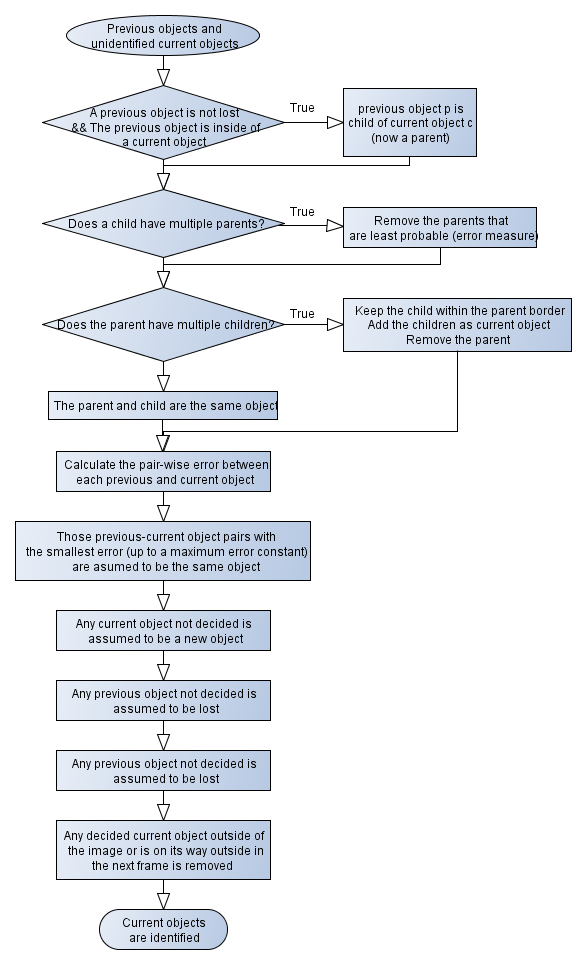
\includegraphics[width=116mm]{images/data_flow_identification.png}
	\caption{\textit{Object Identification flowchart (The 'Ultimate' algorithm).}}
	\label{fig:ObjID_fig} %Skapar referens till figuren
\end{figure}

\subsubsection{Unsolved problems and possible improvements}
TODO...